\subsection{Clamping & Distortion}

Given the voltage ranges of which the amplifying transistors work from (\ref{fig:scope_7}) and (\ref{fig:scope_8}), V_{in-} seems to exhibit a larger swing.
Although we biased these transistors as identically as we could with the current mirrors and DC voltage dividers, they still exhibit some differences.
Notably, the transistor for V_{in-} clearly hits cutoff where the one for V_{in+} does not.
The voltage variation in V_{in+} - V_{in-} was earlier found to be 3.19\si{\volt}
Interestingly, this is approximately equal to V_{DD} - V_{t}, which is the normal limit in voltage output swing for a common-source amplifier.

/FloatBarrier

\begin{figure}[h!]
	\centering
	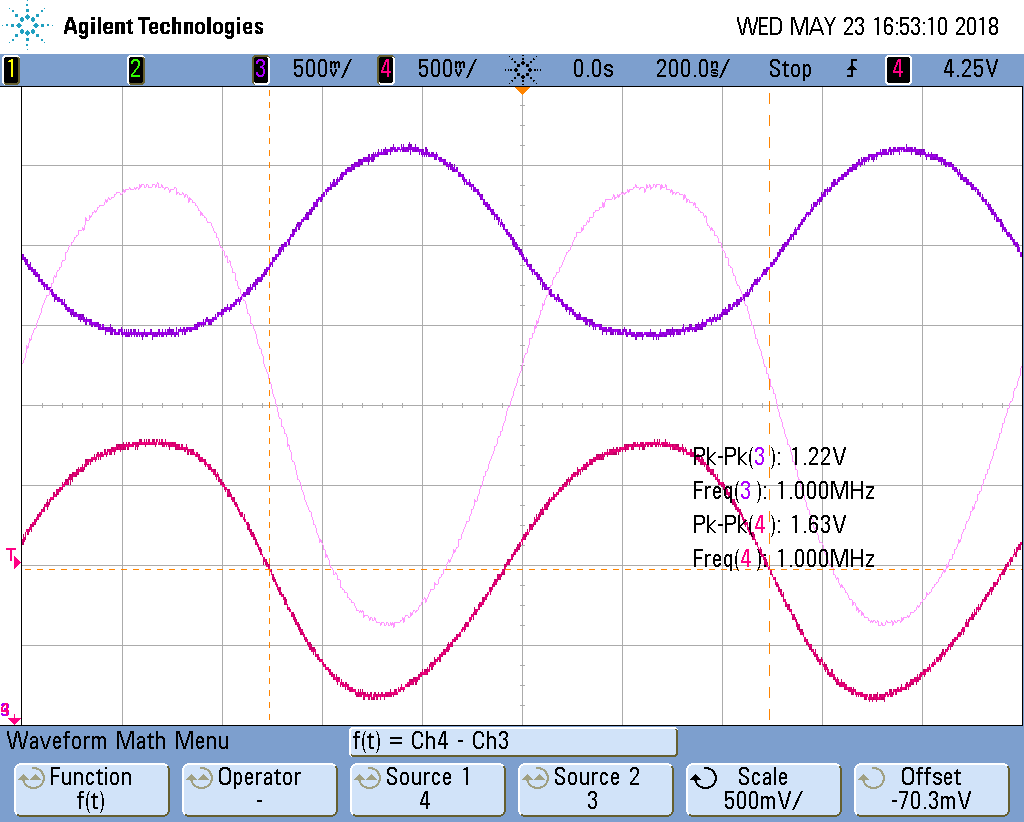
\includegraphics[scale=0.60]{./images/scope_6}
	\caption{Measured maximum signal swing of V_{in+} from a 1.5\si{\volt} p/p input at 1MHz}
	\label{fig:scope_6}
\end{figure}

/FloatBarrier

Therefore, for this differential amplifier, the input signal magnitude should be no greater than 1.5V p/p to avoid significant distortion in signal.
This quantity is similar to the output voltage swing divided by A_{DM}.